\documentclass[11pt]{article}
\usepackage[margin=1in]{geometry}
\usepackage{graphicx}
\usepackage{siunitx}
\usepackage{enumitem}
\usepackage{titlesec}
\setlength{\parindent}{0pt}
\titleformat{\section}{\normalfont\Large\bfseries}{\thesection.}{0.5em}{}

\title{\textbf{Case Study: Why \textit{Titanic} Sank}\\
\large Density, Design and Disaster}
\author{}
\date{}

\begin{document}
\maketitle

\begin{center}
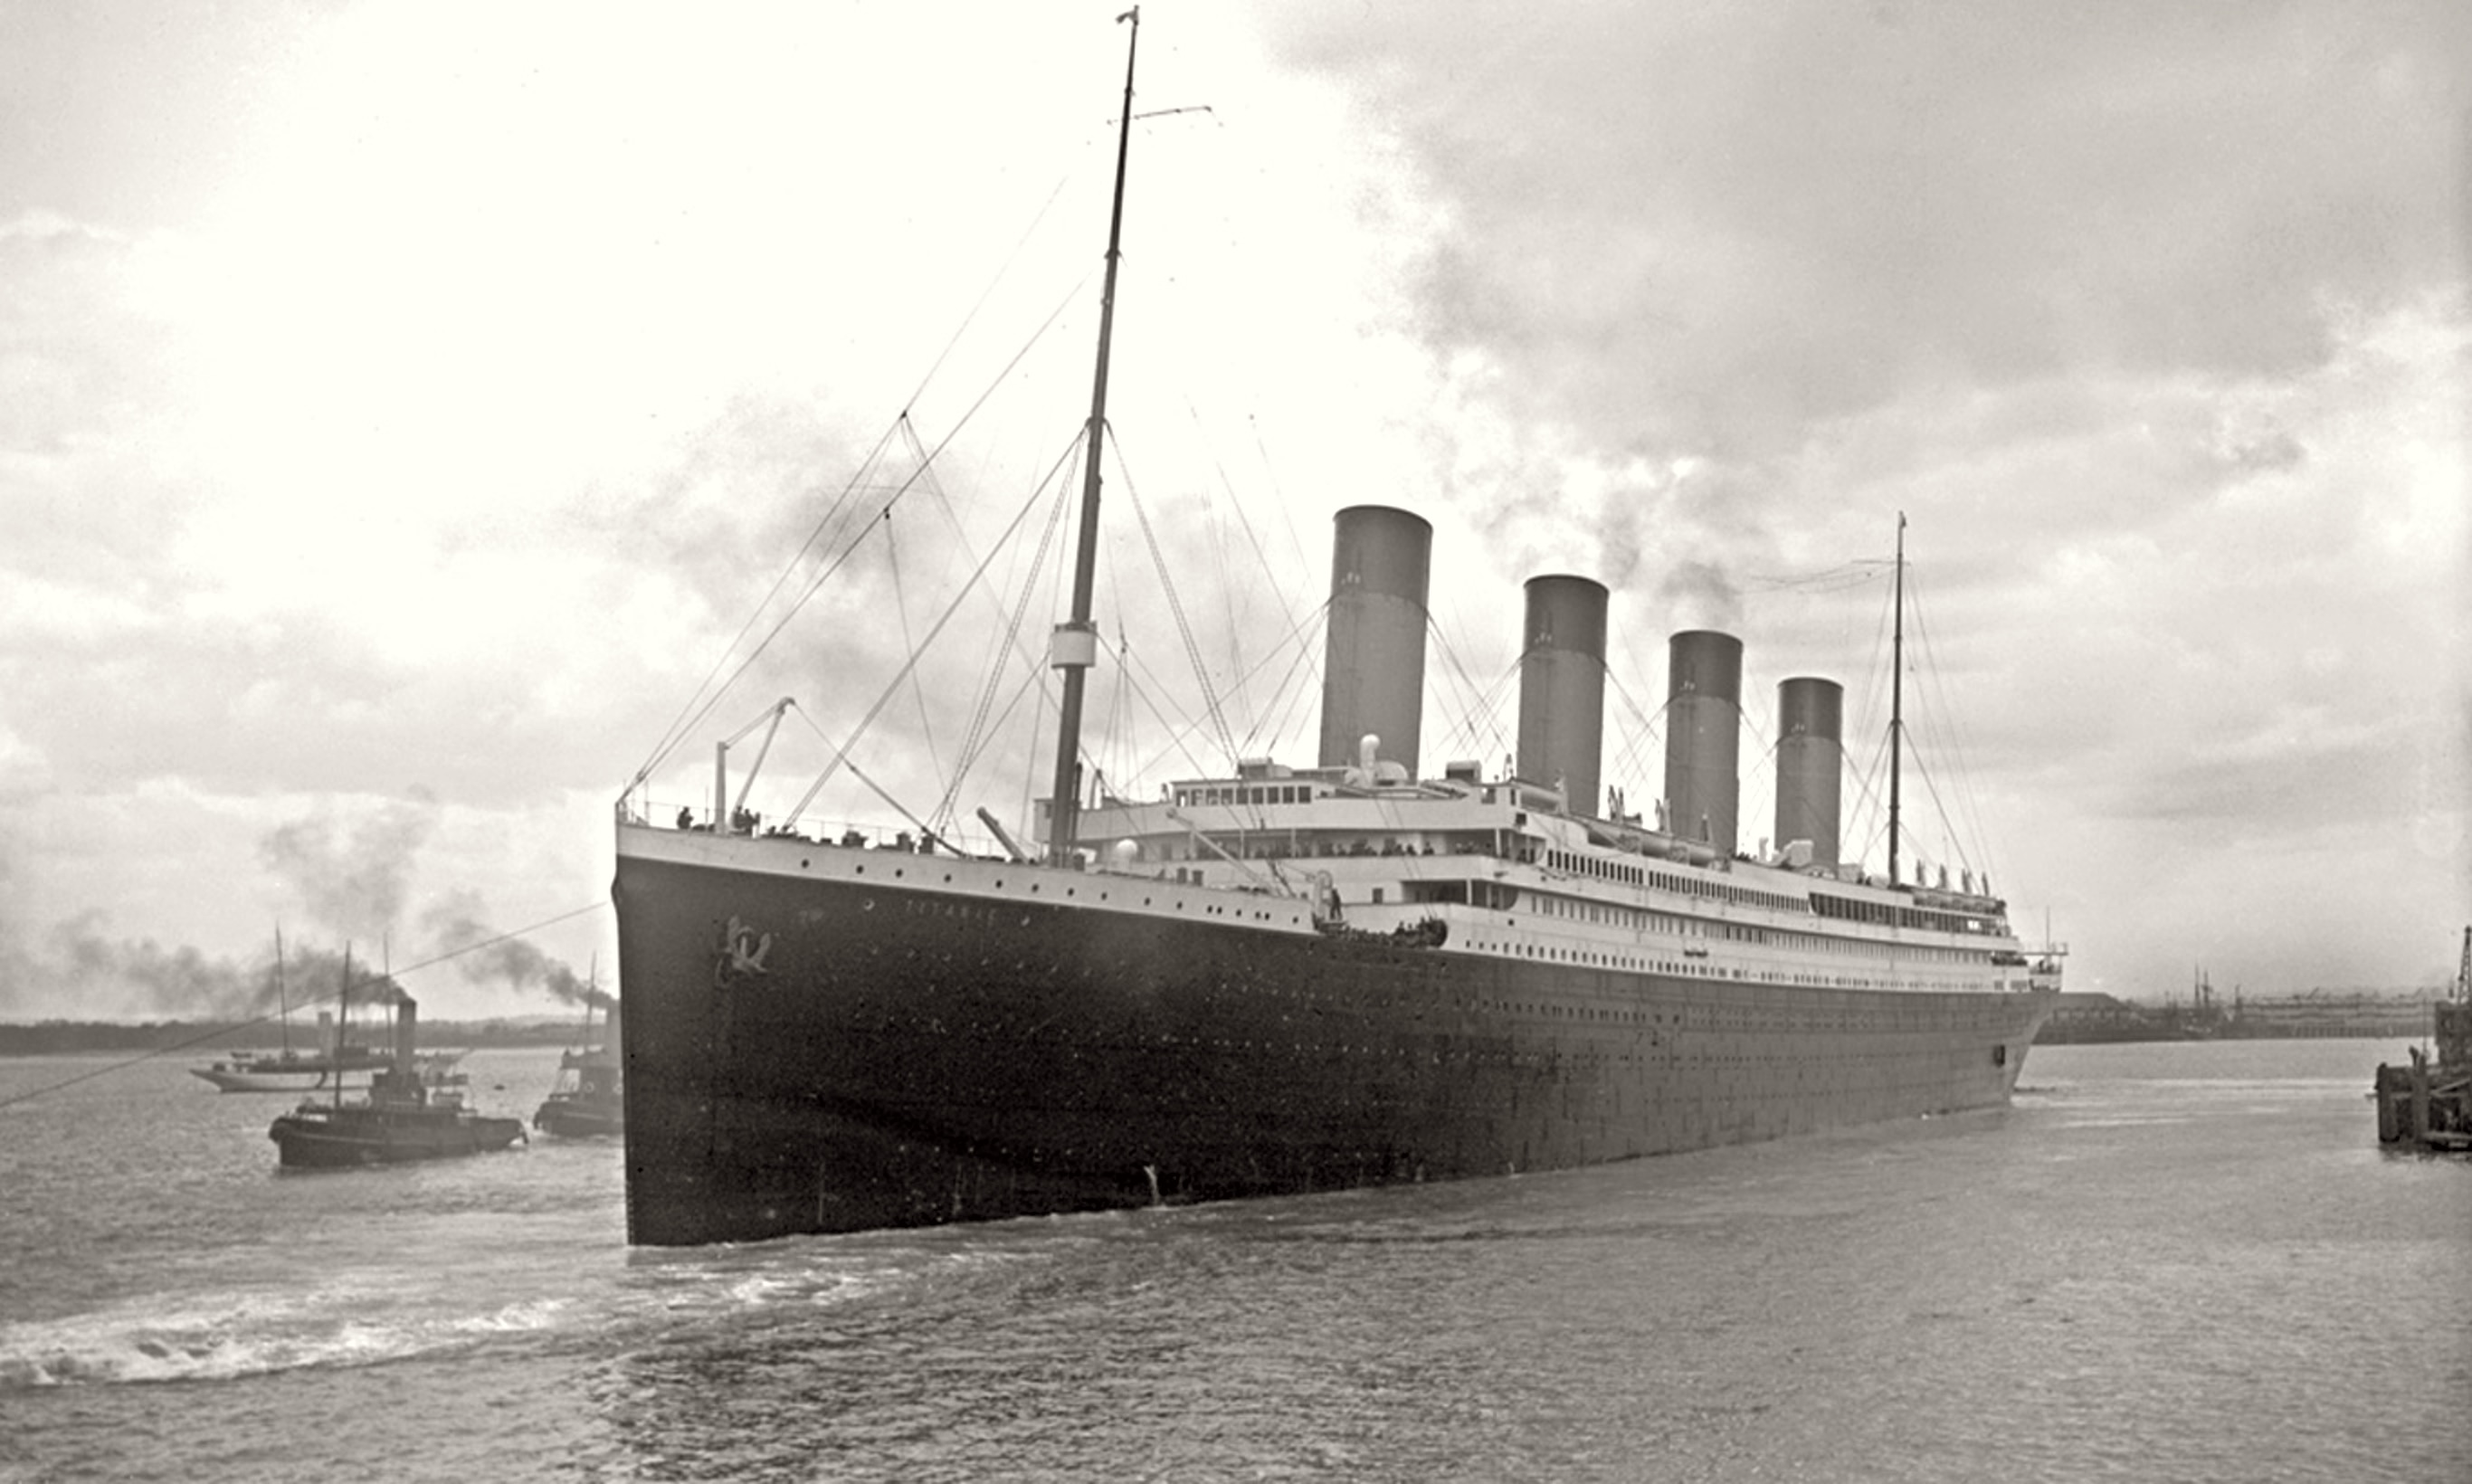
\includegraphics[width=1\linewidth]{titanic_photo.jpg}\\
\emph{Figure 1: RMS \textit{Titanic} leaving Southampton, April 10 1912.}
\end{center}

\section*{Timeline}

\begin{itemize}[leftmargin=*]
\item \textbf{10 Apr 1912\,—\,12:00} Departs Southampton on her maiden voyage. 
\item \textbf{11 Apr 1912\,—\,13:30} Final passenger stop at Queenstown (Cobh), Ireland; heads for New York.
\item \textbf{14 Apr 1912\,—\,21:40} Several ice warnings received; speed maintained at \SI{22}{knots}.
\item \textbf{14 Apr1912\,—\,23:40} Iceberg sighted; starboard collision opens ~\SI{90}{m} of hull plates.
\item \textbf{15 Apr 1912\,—\,00:05} Lifeboat stations ordered; forward holds filling rapidly.
\item \textbf{15 Apr 1912\,—\,02:05} Last lifeboat launched; bow deeply submerged.
\item \textbf{15 Apr 1912\,—\,02:20} \textit{Titanic} breaks apart and sinks. 712 survivors rescued by RMS \textit{Carpathia}.
\end{itemize}

\section{When Density Turns Deadly}

Before the collision, \textit{Titanic} floated because her \textbf{average density}—total mass divided by underwater volume—remained fractionally \emph{lower} than that of seawater. Once the hull was punctured, seawater rushed in, replacing the low‑density air trapped in the forward compartments. Each tonne of water added roughly a tonne of mass without meaningfully increasing the displaced volume, pushing the ship’s average density past the critical \SI{1025}{\kilogram\per\metre^{3}} threshold of North Atlantic seawater.  

\begin{center}
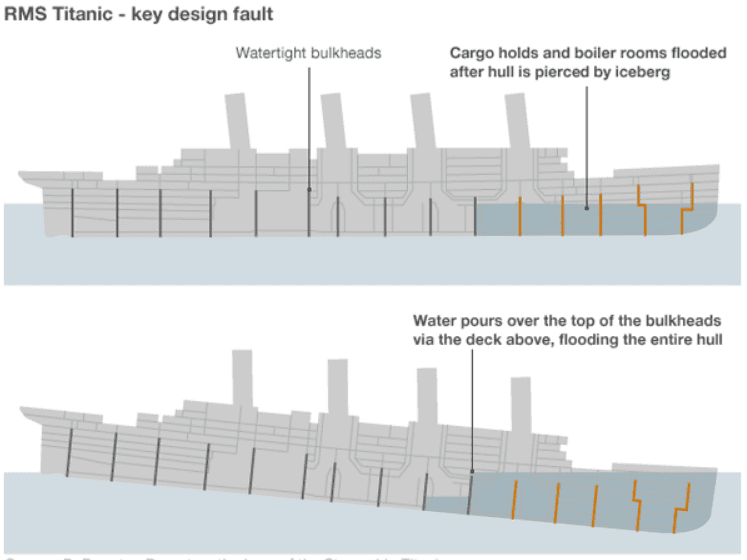
\includegraphics[width=1\linewidth]{compartments_diagram.png}\\
\emph{Figure 2}
\end{center}

Flooding progressed in stages. Bulkheads rose only part‑way to the main deck; as the bow pitched lower, water spilled over into the next compartment, repeating the process until buoyancy was lost completely.

\subsection*{The Density Cascade}

\begin{enumerate}[label=\arabic*.]
\item \textbf{Puncture:} Iceberg tears through plating below the load line.
\item \textbf{Initial Flooding:} Seawater enters at thousands of tonnes per minute; local density at the bow soars.
\item \textbf{Trim Change:} Bow drops, exposing more openings yet adding little extra volume.
\item \textbf{Over‑top Spill:} Water rises above bulkheads not sealed to deck level, flooding successive compartments.
\item \textbf{Critical Density Reached:} Overall density exceeds that of seawater; positive buoyancy is lost and sinking becomes inevitable.
\end{enumerate}

\section{Modern Safeguards Against a Repeat}

Advances in naval architecture target the same density imbalance that doomed \textit{Titanic}. Key measures include:

\begin{itemize}[leftmargin=*]
\item \textbf{Double Hulls \& Side‑Longitudinal Tanks} — An inner shell sits several metres inside the outer plating. A breach in the outer layer floods only a narrow space, keeping the main hull buoyant.
\item \textbf{Full‑Height Watertight Bulkheads} — Subdivision now rises to the main deck (or higher), preventing water from cascading over tops as the vessel trims.
\item \textbf{Transverse \& Longitudinal Subdivision Rules} — Classification societies require finer compartment grids, limiting floodable length so average density cannot exceed seawater even after two adjoining compartments fill.
\item \textbf{High‑Capacity Automatic Pumps} — Redundant, power‑diverse bilge and ballast pumps evacuate floodwater faster than typical inflow from partial breaches.
\item \textbf{Real‑Time Flood Sensors \& Remote Valves} — Crew can seal off damaged zones and monitor water levels from the bridge, stopping density creep early.
\item \textbf{Improved Materials \& Welding} — Modern high‑toughness steel and welded seams resist brittle fracture, reducing the size of openings on impact.
\item \textbf{Ice Detection Radar \& Route Optimisation} — Early warning allows speed reduction and course changes, minimising collision energy.
\end{itemize}

Collectively these features keep a compromised ship’s \emph{average density} below the red line long enough for rescue or self‑recovery.

\newpage
\section*{Questions}

\begin{enumerate}
\item According to the timeline, how long elapsed between the iceberg collision and the ship’s final plunge?
\item Explain why \textit{Titanic} floated before impact yet began to sink once seawater entered the forward compartments.
\item Describe two design shortcomings that allowed water to spread beyond the first five compartments.
\item Why did inflowing seawater increase the vessel’s mass but not its displaced volume appreciably?
\item The North Atlantic that night had a density of roughly \SI{1025}{\kilogram\per\metre^{3}}. If the water had been slightly denser—colder and saltier—would the sinking have been faster, slower, or unchanged? Explain your reasoning.
\item Identify and briefly explain one modern engineering practice that helps prevent a vessel’s average density from exceeding that of seawater after hull damage.
\item \textbf{Extended writing:} “Human judgement was as decisive as physics in the loss of \textit{Titanic}.” Discuss, combining technical factors (density, structural design, speed) with human choices (ice warnings, lifeboat provision, safety culture).
\end{enumerate}

\end{document}
